% Created 2019-10-22 ti 11:10
% Intended LaTeX compiler: pdflatex
\documentclass[12pt]{article}

%%%% settings when exporting code %%%% 

\usepackage{listings}
\lstset{
backgroundcolor=\color{white},
basewidth={0.5em,0.4em},
basicstyle=\ttfamily\small,
breakatwhitespace=false,
breaklines=true,
columns=fullflexible,
commentstyle=\color[rgb]{0.5,0,0.5},
frame=single,
keepspaces=true,
keywordstyle=\color{black},
literate={~}{$\sim$}{1},
numbers=left,
numbersep=10pt,
numberstyle=\ttfamily\tiny\color{gray},
showspaces=false,
showstringspaces=false,
stepnumber=1,
stringstyle=\color[rgb]{0,.5,0},
tabsize=4,
xleftmargin=.23in,
emph={anova,apply,class,coef,colnames,colNames,colSums,dim,dcast,for,ggplot,head,if,ifelse,is.na,lapply,list.files,library,logLik,melt,plot,require,rowSums,sapply,setcolorder,setkey,str,summary,tapply},
emphstyle=\color{blue}
}

%%%% packages %%%%%

\usepackage[utf8]{inputenc}
\usepackage[T1]{fontenc}
\usepackage{lmodern}
\usepackage{textcomp}
\usepackage{color}
\usepackage{enumerate}
\usepackage{graphicx}
\usepackage{grffile}
\usepackage{wrapfig}
\usepackage{rotating}
\usepackage{longtable}
\usepackage{multirow}
\usepackage{multicol}
\usepackage{changes}
\usepackage{pdflscape}
\usepackage{geometry}
\usepackage[normalem]{ulem}
\usepackage{amssymb}
\usepackage{amsmath}
\usepackage{amsfonts}
\usepackage{dsfont}
\usepackage{array}
\usepackage{ifthen}
\usepackage{hyperref}
\usepackage{natbib}
%
%%%% specifications %%%%
%
\usepackage{ifthen}
\usepackage{xifthen}
\usepackage{xargs}
\usepackage{xspace}
\newcommand\Rlogo{\textbf{\textsf{R}}\xspace} %
\RequirePackage{fancyvrb}
\DefineVerbatimEnvironment{verbatim}{Verbatim}{fontsize=\small,formatcom = {\color[rgb]{0.5,0,0}}}
\RequirePackage{colortbl} % arrayrulecolor to mix colors
\RequirePackage{setspace} % to modify the space between lines - incompatible with footnote in beamer
\renewcommand{\baselinestretch}{1.1}
\geometry{top=1cm}
\RequirePackage{epstopdf} % to be able to convert .eps to .pdf image files
\RequirePackage{capt-of} %
\RequirePackage{caption} % newlines in graphics
\RequirePackage{amsmath}
\RequirePackage{algorithm}
\RequirePackage[noend]{algpseudocode}
\RequirePackage{dsfont}
\RequirePackage{amsmath,stmaryrd,graphicx}
\RequirePackage{prodint} % product integral symbol (\PRODI)
\newcommand\defOperator[7]{%
\ifthenelse{\isempty{#2}}{
\ifthenelse{\isempty{#1}}{#7{#3}#4}{#7{#3}#4 \left#5 #1 \right#6}
}{
\ifthenelse{\isempty{#1}}{#7{#3}#4_{#2}}{#7{#3}#4_{#1}\left#5 #2 \right#6}
}
}
\newcommand\defUOperator[5]{%
\ifthenelse{\isempty{#1}}{
#5\left#3 #2 \right#4
}{
\ifthenelse{\isempty{#2}}{\underset{#1}{\operatornamewithlimits{#5}}}{
\underset{#1}{\operatornamewithlimits{#5}}\left#3 #2 \right#4}
}
}
\newcommand{\defBoldVar}[2]{
\ifthenelse{\equal{#2}{T}}{\boldsymbol{#1}}{\mathbf{#1}}
}
\newcommandx\Cov[2][1=,2=]{\defOperator{#1}{#2}{C}{ov}{\lbrack}{\rbrack}{\mathbb}}
\newcommandx\Esp[2][1=,2=]{\defOperator{#1}{#2}{E}{}{\lbrack}{\rbrack}{\mathbb}}
\newcommandx\Prob[2][1=,2=]{\defOperator{#1}{#2}{P}{}{\lbrack}{\rbrack}{\mathbb}}
\newcommandx\Qrob[2][1=,2=]{\defOperator{#1}{#2}{Q}{}{\lbrack}{\rbrack}{\mathbb}}
\newcommandx\Var[2][1=,2=]{\defOperator{#1}{#2}{V}{ar}{\lbrack}{\rbrack}{\mathbb}}
\newcommandx\Binom[2][1=,2=]{\defOperator{#1}{#2}{B}{}{(}{)}{\mathcal}}
\newcommandx\Gaus[2][1=,2=]{\defOperator{#1}{#2}{N}{}{(}{)}{\mathcal}}
\newcommandx\Wishart[2][1=,2=]{\defOperator{#1}{#2}{W}{ishart}{(}{)}{\mathcal}}
\newcommandx\Likelihood[2][1=,2=]{\defOperator{#1}{#2}{L}{}{(}{)}{\mathcal}}
\newcommandx\Information[2][1=,2=]{\defOperator{#1}{#2}{I}{}{(}{)}{\mathcal}}
\newcommandx\Score[2][1=,2=]{\defOperator{#1}{#2}{S}{}{(}{)}{\mathcal}}
\newcommandx\Vois[2][1=,2=]{\defOperator{#1}{#2}{V}{}{(}{)}{\mathcal}}
\newcommandx\IF[2][1=,2=]{\defOperator{#1}{#2}{IF}{}{(}{)}{\mathcal}}
\newcommandx\Ind[1][1=]{\defOperator{}{#1}{1}{}{(}{)}{\mathds}}
\newcommandx\Max[2][1=,2=]{\defUOperator{#1}{#2}{(}{)}{min}}
\newcommandx\Min[2][1=,2=]{\defUOperator{#1}{#2}{(}{)}{max}}
\newcommandx\argMax[2][1=,2=]{\defUOperator{#1}{#2}{(}{)}{argmax}}
\newcommandx\argMin[2][1=,2=]{\defUOperator{#1}{#2}{(}{)}{argmin}}
\newcommandx\cvD[2][1=D,2=n \rightarrow \infty]{\xrightarrow[#2]{#1}}
\newcommandx\Hypothesis[2][1=,2=]{
\ifthenelse{\isempty{#1}}{
\mathcal{H}
}{
\ifthenelse{\isempty{#2}}{
\mathcal{H}_{#1}
}{
\mathcal{H}^{(#2)}_{#1}
}
}
}
\newcommandx\dpartial[4][1=,2=,3=,4=\partial]{
\ifthenelse{\isempty{#3}}{
\frac{#4 #1}{#4 #2}
}{
\left.\frac{#4 #1}{#4 #2}\right\rvert_{#3}
}
}
\newcommandx\dTpartial[3][1=,2=,3=]{\dpartial[#1][#2][#3][d]}
\newcommandx\ddpartial[3][1=,2=,3=]{
\ifthenelse{\isempty{#3}}{
\frac{\partial^{2} #1}{\left( \partial #2\right)^2}
}{
\frac{\partial^2 #1}{\partial #2\partial #3}
}
}
\newcommand\Real{\mathbb{R}}
\newcommand\Rational{\mathbb{Q}}
\newcommand\Natural{\mathbb{N}}
\newcommand\trans[1]{{#1}^\intercal}%\newcommand\trans[1]{{\vphantom{#1}}^\top{#1}}
\newcommand{\independent}{\mathrel{\text{\scalebox{1.5}{$\perp\mkern-10mu\perp$}}}}
\newcommand\half{\frac{1}{2}}
\newcommand\normMax[1]{\left|\left|#1\right|\right|_{max}}
\newcommand\normTwo[1]{\left|\left|#1\right|\right|_{2}}
\author{Brice Ozenne}
\date{\today}
\title{A simple example of multiple imputation using the mice package}
\hypersetup{
 colorlinks=true,
 citecolor=[rgb]{0,0.5,0},
 urlcolor=[rgb]{0,0,0.5},
 linkcolor=[rgb]{0,0,0.5},
 pdfauthor={Brice Ozenne},
 pdftitle={A simple example of multiple imputation using the mice package},
 pdfkeywords={},
 pdfsubject={},
 pdfcreator={Emacs 25.2.1 (Org mode 9.0.4)},
 pdflang={English}
 }
\begin{document}

\maketitle
This document gather code from the documentation of the mice
package. See \url{https://stefvanbuuren.name/mice/}.

\bigskip

Load packages
\lstset{language=r,label= ,caption= ,captionpos=b,numbers=none}
\begin{lstlisting}
library(lava)
library(mice)
library(data.table)
library(ggplot2)
\end{lstlisting}

\section{Simulate data (just to have an example to work with)}
\label{sec:org9e85ddf}
Generative model
\lstset{language=r,label= ,caption= ,captionpos=b,numbers=none}
\begin{lstlisting}
mSim <- lvm(Y~group+season+bmi+gender+age)
categorical(mSim, labels = c("winter","summer")) <- ~season
categorical(mSim, labels = c("SAD","HC")) <- ~group
categorical(mSim, labels = c("Male","Female")) <- ~gender
distribution(mSim,~bmi) <- lava::gaussian.lvm(mean = 22, sd = 3)
distribution(mSim,~age) <- lava::uniform.lvm(20,80)
\end{lstlisting}

Sampling
\lstset{language=r,label= ,caption= ,captionpos=b,numbers=none}
\begin{lstlisting}
n <- 1e2
set.seed(10)
dt.data <- as.data.table(sim(mSim,n))
\end{lstlisting}

Add missing values
\lstset{language=r,label= ,caption= ,captionpos=b,numbers=none}
\begin{lstlisting}
dt.data[1:10, bmi:=NA]
\end{lstlisting}

\clearpage

\section{Working with mice}
\label{sec:org37e734f}

\subsection{Step 1: Inspect the missing data pattern}
\label{sec:org59c8972}
Check the number of missing values in the dataset:
\lstset{language=r,label= ,caption= ,captionpos=b,numbers=none}
\begin{lstlisting}
colSums(is.na(dt.data))
\end{lstlisting}

\begin{verbatim}
Y  group season    bmi gender    age 
0      0      0     10      0      0
\end{verbatim}

Missing data patterns:   
\lstset{language=r,label= ,caption= ,captionpos=b,numbers=none}
\begin{lstlisting}
md.pattern(dt.data)
\end{lstlisting}

\begin{center}
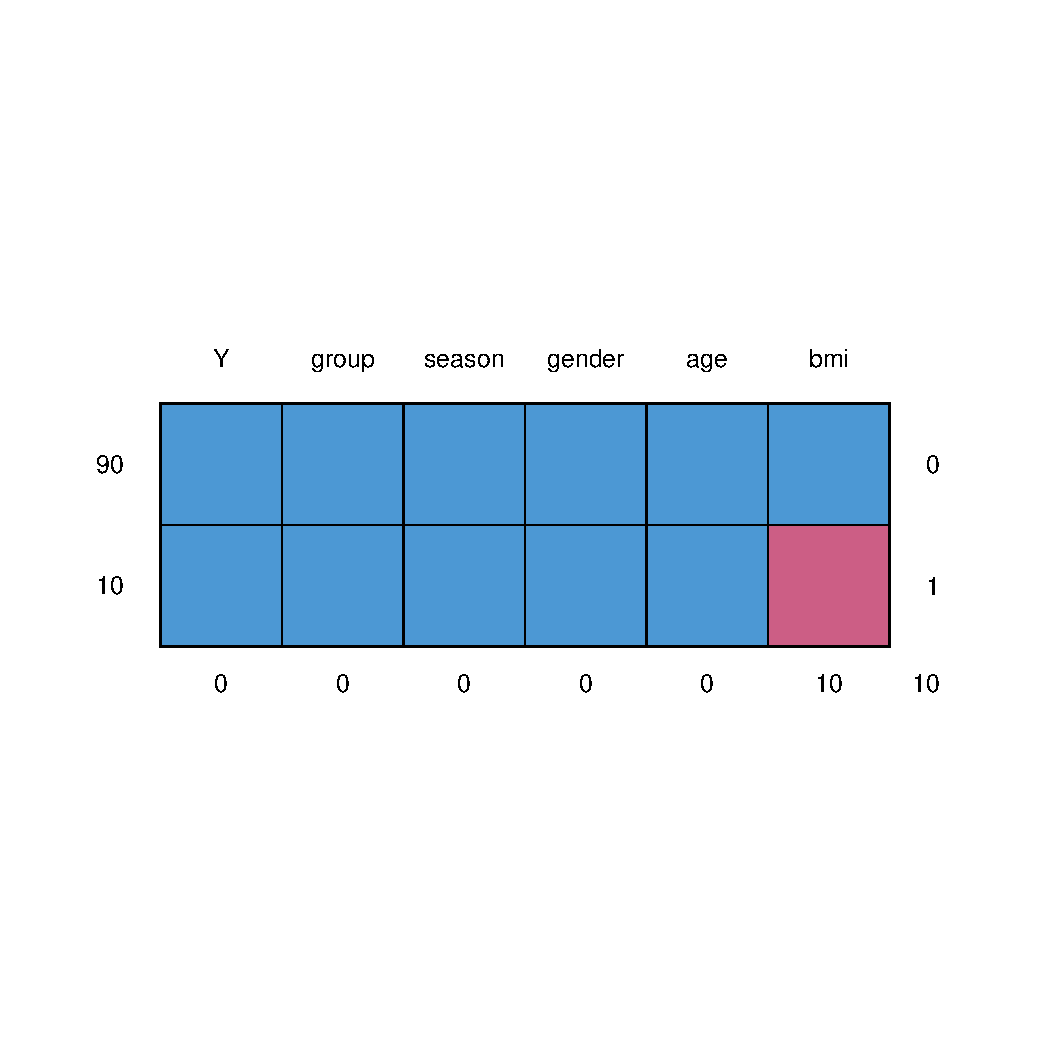
\includegraphics[width=.9\linewidth]{./missingDataPattern.pdf}
\end{center}

\clearpage

\subsection{Step 2: Define imputation model}
\label{sec:org3ca7387}

\lstset{language=r,label= ,caption= ,captionpos=b,numbers=none}
\begin{lstlisting}
all.variables <- c("Y","group","season","bmi","gender","age")
n.variables <- length(all.variables)
Mlink <- matrix(0, n.variables, n.variables,
				dimnames = list(all.variables,all.variables))
Mlink[c("group","season","gender","age"),"bmi"] <- 1
Mlink
\end{lstlisting}

\begin{verbatim}
       Y group season bmi gender age
Y      0     0      0   0      0   0
group  0     0      0   1      0   0
season 0     0      0   1      0   0
bmi    0     0      0   0      0   0
gender 0     0      0   1      0   0
age    0     0      0   1      0   0
\end{verbatim}

A value 1 indicates that the column variable was used to impute the
row variable, e.g. group was used to impute bmi.

\clearpage

\subsection{Step 3: Generate imputed datasets}
\label{sec:orgef4a2e5}
Generate imputed values
\lstset{language=r,label= ,caption= ,captionpos=b,numbers=none}
\begin{lstlisting}
n.imputed <- 3 ## number of imputed datasets
dt.mice <- mice(dt.data,
				m=n.imputed, 
				maxit = 50, # number of iterations to obtain the imputed dataset
				predictorMatrix = Mlink,
				method = 'pmm', # Predictive mean matching, only ok for continuous variables, it is possible to set constrains for positive variables
				seed = 500, printFlag = FALSE)
summary(dt.mice)
\end{lstlisting}

\begin{verbatim}
Class: mids
Number of multiple imputations:  3 
Imputation methods:
     Y  group season    bmi gender    age 
    ""     ""     ""  "pmm"     ""     "" 
PredictorMatrix:
       Y group season bmi gender age
Y      0     0      0   0      0   0
group  0     0      0   1      0   0
season 0     0      0   1      0   0
bmi    0     0      0   0      0   0
gender 0     0      0   1      0   0
age    0     0      0   1      0   0
\end{verbatim}

\clearpage

\subsection{Step 4: Check the imputed datasets}
\label{sec:orga49f6c5}
\subsubsection{Convergence of the imputation algorithm}
\label{sec:orgf31e1b7}

\lstset{language=r,label= ,caption= ,captionpos=b,numbers=none}
\begin{lstlisting}
plot(dt.mice)
\end{lstlisting}

\begin{center}
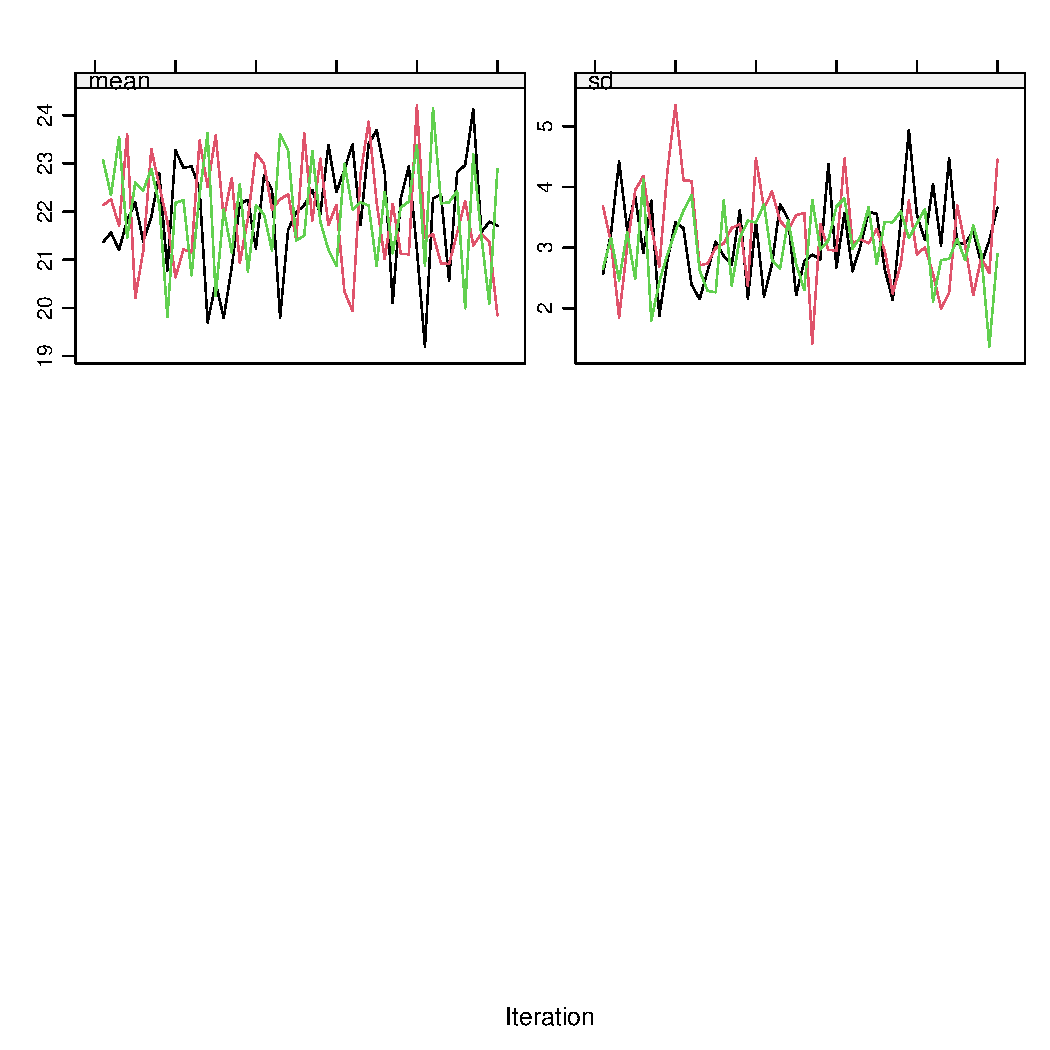
\includegraphics[width=.9\linewidth]{./traceCVimputed.pdf}
\end{center}

\subsubsection{Visualizing the imputed values}
\label{sec:org6fb57d8}
Visualize imputed value values and check they are plausible (e.g. mice
is not imputed a BMI of 75):
\lstset{language=r,label= ,caption= ,captionpos=b,numbers=none}
\begin{lstlisting}
dt.mice$imp$bmi
\end{lstlisting}

\begin{verbatim}
          1        2        3
1  20.15124 21.82216 20.90548
2  25.74547 24.76365 25.98147
3  21.27058 15.52519 26.41881
4  14.44499 23.83614 24.66090
5  24.51607 25.74547 21.08652
6  26.55555 22.05849 24.51607
7  20.97076 20.69408 25.02349
8  22.17178 17.51962 24.76365
9  17.60500 21.94247 26.41881
10 18.25130 22.05849 25.69917
\end{verbatim}

The rows correspond to the 3 different imputed datasets and the
columns to 10 imputed values per dataset. One can also summarizes the
imputed values computing their quantiles:

\lstset{language=r,label= ,caption= ,captionpos=b,numbers=none}
\begin{lstlisting}
apply(dt.mice$imp$bmi,2,quantile)
\end{lstlisting}

\begin{verbatim}
            1        2        3
0%   14.44499 15.52519 20.90548
25%  18.72629 20.97610 24.55228
50%  21.12067 22.00048 24.89357
75%  23.93000 23.39173 25.91090
100% 26.55555 25.74547 26.41881
\end{verbatim}

Boxplot of the imputed values:

\lstset{language=r,label= ,caption= ,captionpos=b,numbers=none}
\begin{lstlisting}
boxplot(dt.mice$imp$bmi)
\end{lstlisting}

\begin{center}
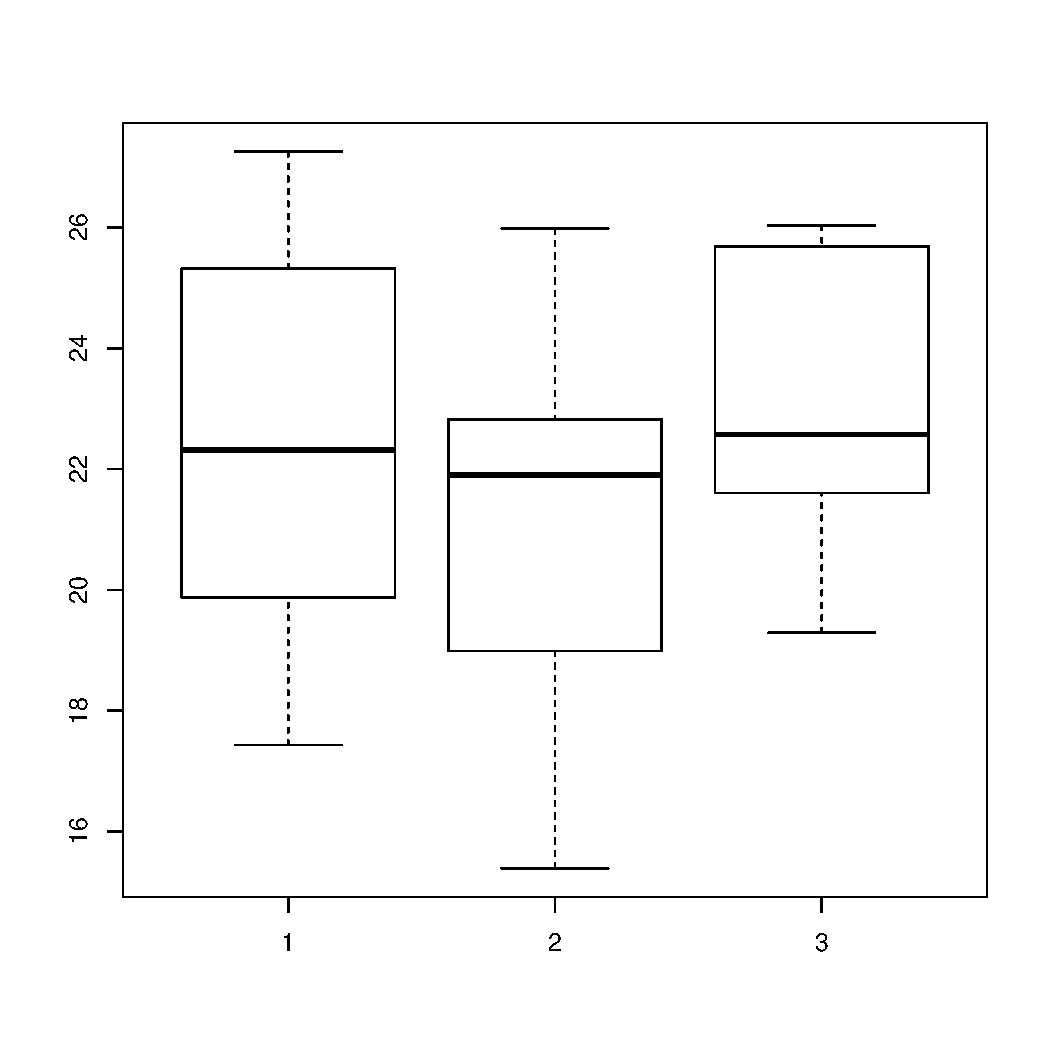
\includegraphics[width=.9\linewidth]{./boxplotImputed.pdf}
\end{center}

Imputed values vs. observed values
\lstset{language=r,label= ,caption= ,captionpos=b,numbers=none}
\begin{lstlisting}
dt.bmi <- rbind(data.table(bmi = unlist(dt.mice$imp$bmi), imputed = TRUE),
				data.table(bmi = na.omit(dt.data$bmi), imputed = FALSE))
\end{lstlisting}

Histogram
\lstset{language=r,label= ,caption= ,captionpos=b,numbers=none}
\begin{lstlisting}
gg1.bmi <- ggplot(dt.bmi, aes(bmi, group = imputed, fill = imputed))
gg1.bmi <- gg1.bmi + geom_histogram(aes(y=..count../sum(..count..)),position = "dodge")
gg1.bmi
\end{lstlisting}

\begin{verbatim}
`stat_bin()` using `bins = 30`. Pick better value with `binwidth`.
\end{verbatim}

\begin{center}
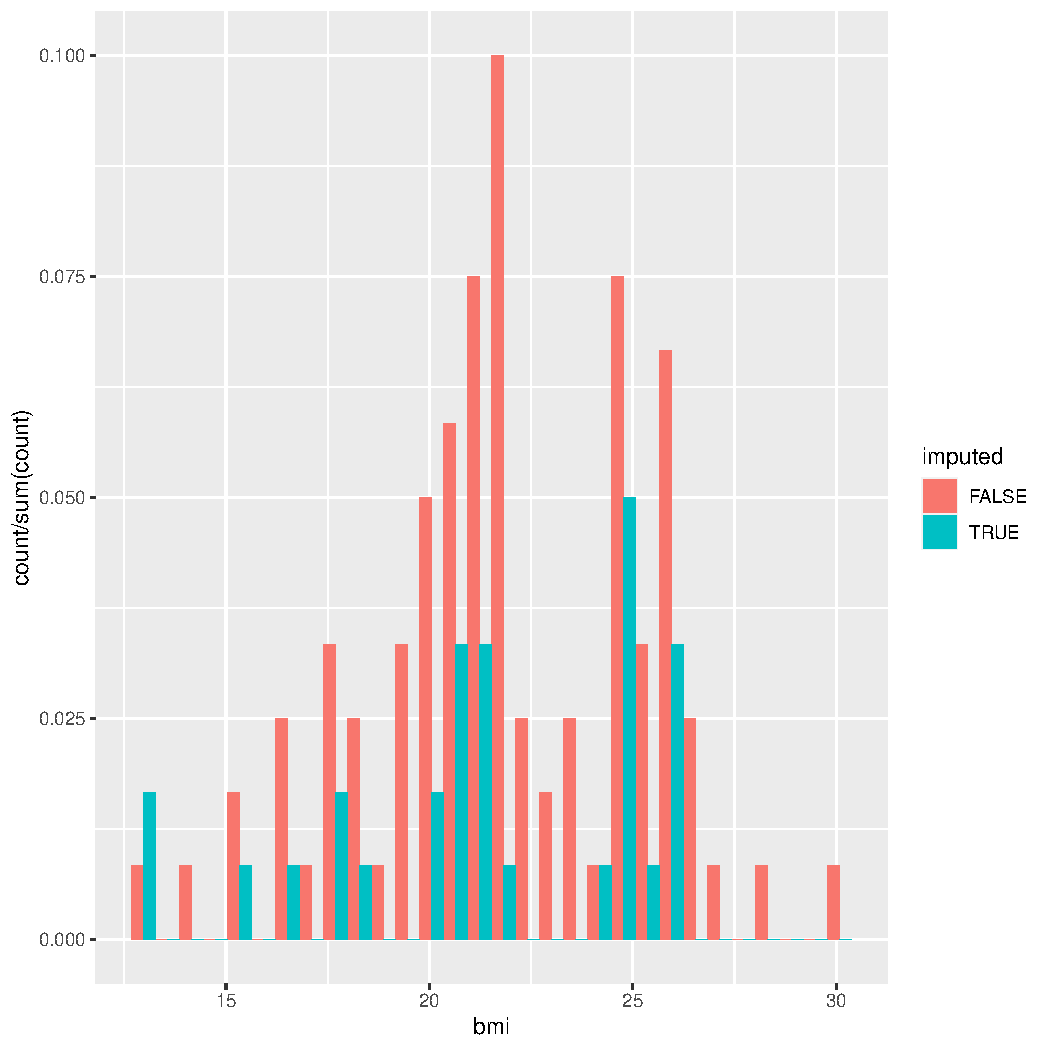
\includegraphics[width=.9\linewidth]{./histImputed.pdf}
\end{center}

One more plot:

\lstset{language=r,label= ,caption= ,captionpos=b,numbers=none}
\begin{lstlisting}
stripplot(dt.mice, bmi~.imp, pch=20, cex=2)
\end{lstlisting}

\begin{center}
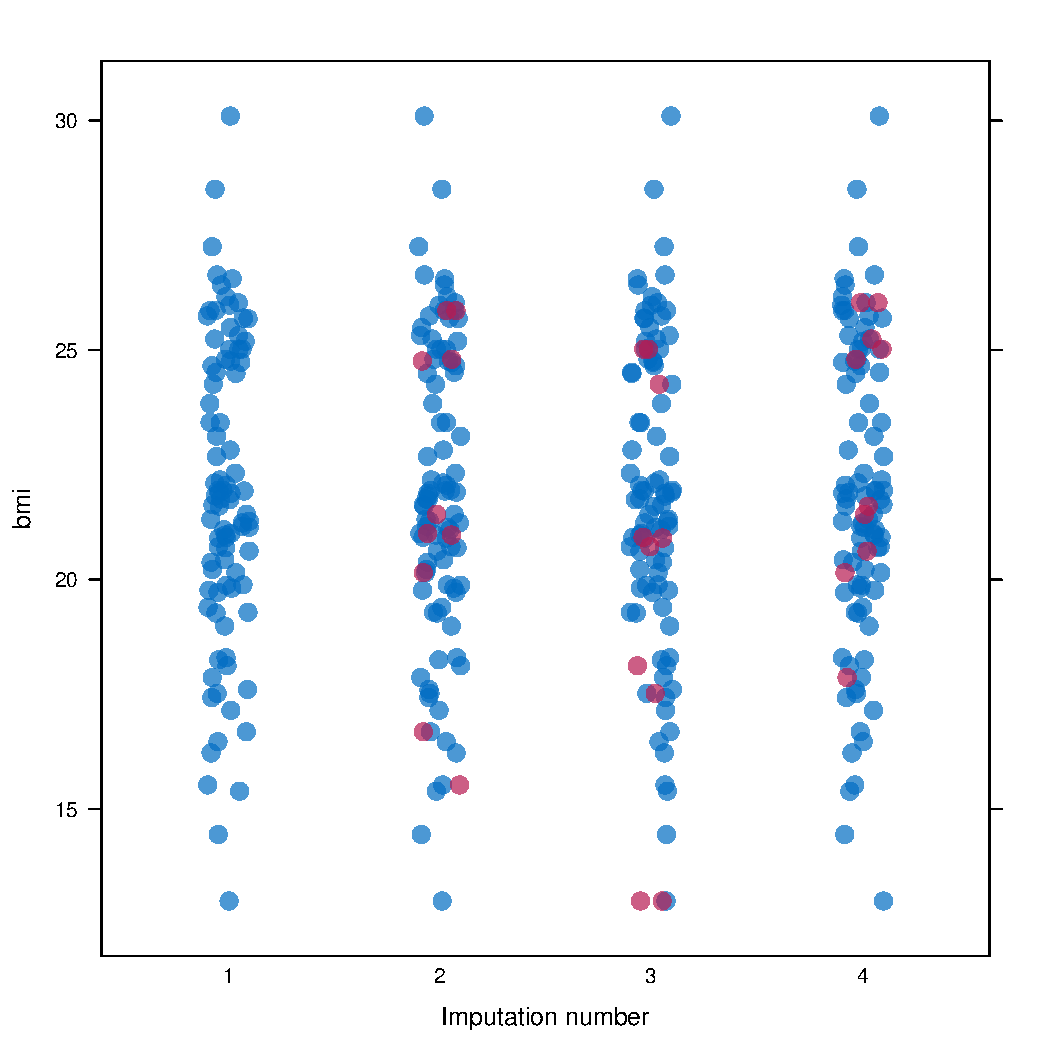
\includegraphics[width=.9\linewidth]{./striplotImputed.pdf}
\end{center}

\clearpage

\subsection{Step 3: Fit the statical model on each imputed dataset}
\label{sec:org7e31945}

\lstset{language=r,label= ,caption= ,captionpos=b,numbers=none}
\begin{lstlisting}
e.mice <- with(data = dt.mice,
			   lm(Y~group+season+bmi+gender+age)
			   )
e.mice
\end{lstlisting}

\begin{verbatim}
call :
with.mids(data = dt.mice, expr = lm(Y ~ group + season + bmi + 
    gender + age))

call1 :
mice(data = dt.data, m = n.imputed, method = "pmm", predictorMatrix = Mlink, 
    maxit = 50, printFlag = FALSE, seed = 500)

nmis :
     Y  group season    bmi gender    age 
     0      0      0     10      0      0 

analyses :
[[1]]

Call:
lm(formula = Y ~ group + season + bmi + gender + age)

Coefficients:
 (Intercept)       groupHC  seasonsummer           bmi  genderFemale           age  
      2.6716        0.7320        1.1417        0.8566        0.6350        1.0124  


[[2]]

Call:
lm(formula = Y ~ group + season + bmi + gender + age)

Coefficients:
 (Intercept)       groupHC  seasonsummer           bmi  genderFemale           age  
      2.1738        0.4821        1.2057        0.9066        0.6046        1.0020  


[[3]]

Call:
lm(formula = Y ~ group + season + bmi + gender + age)

Coefficients:
 (Intercept)       groupHC  seasonsummer           bmi  genderFemale           age  
      1.4529        0.3860        1.1272        0.9050        0.9807        1.0094
\end{verbatim}

Check that using \texttt{with}:
\lstset{language=r,label= ,caption= ,captionpos=b,numbers=none}
\begin{lstlisting}
e.mice$analyses[[1]]
\end{lstlisting}

\begin{verbatim}

Call:
lm(formula = Y ~ group + season + bmi + gender + age)

Coefficients:
 (Intercept)       groupHC  seasonsummer           bmi  genderFemale           age  
      2.6716        0.7320        1.1417        0.8566        0.6350        1.0124
\end{verbatim}

is equivalent to run the linear regression on the imputed dataset:
\lstset{language=r,label= ,caption= ,captionpos=b,numbers=none}
\begin{lstlisting}
dt.tempo <- copy(dt.data)
dt.tempo[is.na(bmi), bmi := dt.mice$imp$bmi[,1]]
lm(Y ~ group + season + bmi + gender + age, data  = dt.tempo)
\end{lstlisting}

\begin{verbatim}

Call:
lm(formula = Y ~ group + season + bmi + gender + age, data = dt.tempo)

Coefficients:
 (Intercept)       groupHC  seasonsummer           bmi  genderFemale           age  
      2.6716        0.7320        1.1417        0.8566        0.6350        1.0124
\end{verbatim}

\clearpage

\subsection{Step 4: Pool the results over the imputed datasets}
\label{sec:org16ce1fb}

\lstset{language=r,label= ,caption= ,captionpos=b,numbers=none}
\begin{lstlisting}
ePool.mice <- pool(e.mice)
summary(ePool.mice)
\end{lstlisting}

\begin{verbatim}
              estimate  std.error statistic       df     p.value
(Intercept)  2.0994178 1.53720448  1.365737 27.60999 0.175443034
groupHC      0.5333769 0.42990642  1.240681 24.64629 0.217965151
seasonsummer 1.1581844 0.37942876  3.052442 89.52004 0.002988004
bmi          0.8894300 0.06542205 13.595263 21.64939 0.000000000
genderFemale 0.7401163 0.44568379  1.660631 17.16642 0.100286406
age          1.0079300 0.01217062 82.816644 20.68587 0.000000000
\end{verbatim}


The (pooled) estimate is the average of the estimates relative to each
imputed dataset:
\lstset{language=r,label= ,caption= ,captionpos=b,numbers=none}
\begin{lstlisting}
Q.coef <- colMeans(do.call(rbind,lapply(e.mice$analyses, coef)))
Q.coef
\end{lstlisting}

\begin{verbatim}
(Intercept)      groupHC seasonsummer          bmi genderFemale          age 
  2.0994178    0.5333769    1.1581844    0.8894300    0.7401163    1.0079300
\end{verbatim}

The variance is a bit more complex and involves:
\begin{itemize}
\item the within-imputation variance (depends on the sample size)
\end{itemize}
\lstset{language=r,label= ,caption= ,captionpos=b,numbers=none}
\begin{lstlisting}
covW <- Reduce("+",lapply(e.mice$analyses, vcov))/n.imputed
covW
\end{lstlisting}

\begin{verbatim}
              (Intercept)       groupHC  seasonsummer           bmi  genderFemale           age
(Intercept)   1.862431644 -0.0994440642 -0.0477903745 -6.786768e-02 -0.0961541467 -4.196538e-03
groupHC      -0.099444064  0.1422982153  0.0119430572  2.070599e-03  0.0056222025 -5.605698e-04
seasonsummer -0.047790374  0.0119430572  0.1416426832 -1.604466e-03  0.0129427682 -1.624194e-04
bmi          -0.067867684  0.0020705988 -0.0016044660  3.202784e-03 -0.0001538781 -4.848575e-05
genderFemale -0.096154147  0.0056222025  0.0129427682 -1.538781e-04  0.1404564390  2.433642e-04
age          -0.004196538 -0.0005605698 -0.0001624194 -4.848575e-05  0.0002433642  1.096841e-04
\end{verbatim}

\begin{itemize}
\item the between-imputation variance (depends on the amount of missin data)
\end{itemize}
\lstset{language=r,label= ,caption= ,captionpos=b,numbers=none}
\begin{lstlisting}
ls.diffCoef <- lapply(e.mice$analyses, function(iI){coef(iI)-Q.coef})
covB <- Reduce("+",lapply(ls.diffCoef,tcrossprod))/(n.imputed-1)
covB
\end{lstlisting}

\begin{verbatim}
              [,1]          [,2]          [,3]          [,4]          [,5]          [,6]
[1,]  0.3754244681  0.1025439091  0.0070478503 -0.0137914086 -0.1128631208  5.705877e-04
[2,]  0.1025439091  0.0318909867 -0.0005751962 -0.0048485267 -0.0246900921  4.853229e-04
[3,]  0.0070478503 -0.0005751962  0.0017426263  0.0004376612 -0.0060716948 -2.014883e-04
[4,] -0.0137914086 -0.0048485267  0.0004376612  0.0008079455  0.0024361901 -1.127512e-04
[5,] -0.1128631208 -0.0246900921 -0.0060716948  0.0024361901  0.0436332030  3.493617e-04
[6,]  0.0005705877  0.0004853229 -0.0002014883 -0.0001127512  0.0003493617  2.882992e-05
\end{verbatim}

\begin{itemize}
\item the simulation error
\end{itemize}
\lstset{language=r,label= ,caption= ,captionpos=b,numbers=none}
\begin{lstlisting}
covE <- covB/n.imputed
covE
\end{lstlisting}

\begin{verbatim}
              [,1]          [,2]          [,3]          [,4]          [,5]          [,6]
[1,]  0.1251414894  0.0341813030  2.349283e-03 -4.597136e-03 -0.0376210403  1.901959e-04
[2,]  0.0341813030  0.0106303289 -1.917321e-04 -1.616176e-03 -0.0082300307  1.617743e-04
[3,]  0.0023492834 -0.0001917321  5.808754e-04  1.458871e-04 -0.0020238983 -6.716278e-05
[4,] -0.0045971362 -0.0016161756  1.458871e-04  2.693152e-04  0.0008120634 -3.758374e-05
[5,] -0.0376210403 -0.0082300307 -2.023898e-03  8.120634e-04  0.0145444010  1.164539e-04
[6,]  0.0001901959  0.0001617743 -6.716278e-05 -3.758374e-05  0.0001164539  9.609975e-06
\end{verbatim}

The total variance is:
\lstset{language=r,label= ,caption= ,captionpos=b,numbers=none}
\begin{lstlisting}
covT <- covW + covB + covE
\end{lstlisting}

leading to the standard errors:
\lstset{language=r,label= ,caption= ,captionpos=b,numbers=none}
\begin{lstlisting}
sqrt(diag(covT))
\end{lstlisting}
\begin{verbatim}
(Intercept)      groupHC seasonsummer          bmi genderFemale          age 
 1.53720448   0.42990642   0.37942876   0.06542205   0.44568379   0.01217062
\end{verbatim}

\clearpage

\section{Reporting guideline}
\label{sec:orgf206599}
From \url{https://stefvanbuuren.name/Winnipeg/Lectures/Winnipeg.pdf}:
\begin{itemize}
\item Amount of missing data
\item Reasons for missingness
\item Differences between complete and incomplete data
\item Method used to account for missing data
\item Software
\item Number of imputed datasets
\item Imputation model
\item Derived variables
\item Diagnostics
\item Pooling
\item Listwise deletion
\item Sensitivity analysis
\end{itemize}
\end{document}